\section{Background}

In this section, we review the topics that will be used as building blocks for the remainder of the chapter. 
First, we discuss the details of debloating web applications based on dynamic code-coverage traces. 
Then, we review several source code metrics that can be used to measure the effectiveness of debloating from the perspective of attack-surface reduction.

\begin{figure}[t]
    \centering
    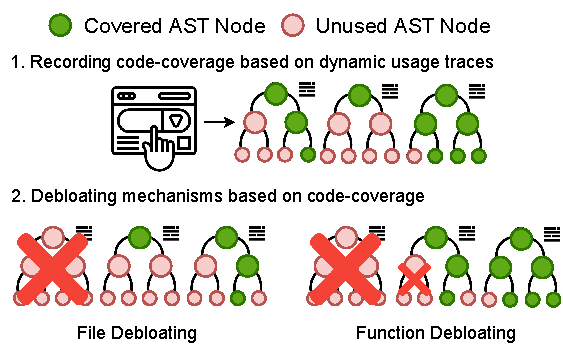
\includegraphics[width=0.75\columnwidth]{figures/dbltr/file_vs_function_debloating.drawio.pdf}
    \caption{File vs Function level debloating based on dynamic code-coverage traces. Root of each AST denotes the entry point of the underlying PHP file. Second layer nodes denote functions, and the leaves are statements inside functions.}
    \label{fig:file_vs_func_debloating}
\end{figure}

\subsection{Debloating based on dynamic usage traces}
Debloating based on dynamic traces for web applications was first introduced in ``Less is More''~\cite{lessismore}, in which we incorporate a set of automation tools and scripts to \emph{simulate} usage behavior while recording the executed server-side files as well as their respective lines.
Figure~\ref{fig:file_vs_func_debloating} represents the two debloating approaches discussed by ``Less is More''~\cite{lessismore}. 
Based on this code-coverage information (Step 1 in Figure~\ref{fig:file_vs_func_debloating}) ``Less is More'' identifies unused nodes in the Abstract Syntax Tree (AST). 

In ``Less is More'' we discussed two debloating strategies, file-level and function-level debloating. 
In the first approach, file debloating only removes the whole AST of a file, if none of its underlying statements are ever exercised based on the dynamic usage traces. 
Conversely, function debloating is fine-grained and can remove sub-graphs of the AST if it identifies a function with no code-coverage, and therefore, can produce smaller applications with fewer vulnerabilities. 

``Less is More'' incorporates the XDebug PHP module that allows it to record the list of executed PHP file and lines. 
Next step is to configure the web server to start XDebug for each of the running PHP files. 
By configuring XDebug to run for each PHP file invoked by the web server, ``Less is More'' records the list of PHP files and their underlying executed lines and stores them in a database. 
In this work, we follow a similar method to record the code-coverage, and extend ``Less is More'' by looking at \emph{real} user data, and identifying clusters of users that perform similar actions. 

\subsection{Debloating metrics}

Debloating by definition removes or neutralizes parts of the application that users do not require. 
In order to demonstrate the security gains by removing a piece of code, previous work has used several source-code metrics. 

\paragraph{Size reduction} measures how much code was removed through the debloating process. 
McConnell discussed in his work that the size of the code positively correlates with the number of software bugs it contains~\cite{mcconnell2004code}. The reduction in Logical Lines of Code (LLOC) measures the size reduction by counting the number of statements in an application pre-~and post-debloating and is resilient to changes in the syntax and coding style.

\paragraph{Reduction of security vulnerabilities} is another metric that focuses on historic CVEs. 
By mapping public CVEs to the source code of web applications, we can identify whether the vulnerable piece of code is removed by debloating. 
This is a powerful metric as it focuses on real and mostly exploitable vulnerabilities as opposed to proxy variables (such as LLOC) that may or may not result in real vulnerabilities. In terms of downsides, next to the effort required to map vulnerabilities to source code, CVE-reduction is only meaningful in hindsight since it can be used to understand how a debloating system would have performed if an application was debloated \emph{before} the now-known vulnerabilities were discovered. 


\paragraph{Critical API Calls (CAC) reduction} 
PHP applications interact with their environment through the APIs provided by the PHP engine, which are also known as built-in functions. 
These functions expose low-level C API implementations and provide a variety of functionality to perform network, database, and file-system operations. 
Similarly, PHP extensions which are also written in C, expose their functionality through defining new APIs. 

Protecting CACs has received the attention of binary debloating and exploit prevention research in the past. 
Namely, Shredder~\cite{mishra2018shredder}, ROPGuard~\cite{fratric2012ropguard}, and kBouncer~\cite{pappas2012kbouncer} have emphasized the importance of protecting Critical APIs. 
In the realm of web applications, the prior work on taint analysis for vulnerability detection commonly incorporates the list of such critical APIs that attackers can use to execute various types of attacks. 
For instance, attackers can abuse APIs exposed through the MySQLi PHP extension to mount SQL injection attacks. 
Similarly, the exploitation of file-system APIs can lead to arbitrary file-write attacks. 
Therefore, reducing the access of attackers to such functions through debloating provides tangible security benefits. The RIPS tool by Dahse et al. provided a comprehensive list of Critical APIs, which were treated as sinks for PHP taint analysis~\cite{dahse2010rips}. 
We incorporate the 205 sinks from RIPS and measure the removal of such critical API calls (CACs) from the debloated web applications. 

We categorize the sensitive sinks from RIPS into four main groups. \textbf{Code Execution APIs} are those which can be used to directly, or indirectly run code or change the control flow of the application (e.g., call an arbitrary function). 
Next on this list are \textbf{File System APIs} which enable interactions with the file system, such as, deletion and file manipulation and can be abused to take over an application by overwriting files, overriding credentials, and removing sensitive configuration files. 
\textbf{Information Disclosure} functions can be abused by attackers to expose sensitive information from the web application or its host operating system. 
Lastly, for APIs that do not clearly belong to one of the aforementioned categories, we list them under \textbf{Other}. 
This group of critical APIs may allow attackers to conduct malicious actions, such as, sending spam emails, or evading authentication by changing environment variables. 
Next, we look at some examples from each of these categories of critical APIs: 

\begin{itemize}
    \item \textbf{Code Execution APIs:} Consist of OS Shell command execution (e.g., \texttt{exec}, \texttt{passthru}, \texttt{popen}, etc.) PHP code execution (e.g., \texttt{eval}, \texttt{assert}, etc.) and Callbacks (e.g., \texttt{call\_user\_func, array\_map}, etc.)
    \item \textbf{File System APIs :} Consist of functions such as \texttt{fopen}, \texttt{file\_put\_contents}, and \texttt{rename}.
    \item \textbf{Information Disclosure APIs:} Include functions that can leak sensitive information from the web server environment such as \texttt{getenv}, \texttt{get\_current\_user}, and \texttt{phpinfo}.
    \item \textbf{Other APIs:} This group consists of miscellaneous critical APIs such as \texttt{extract}, \texttt{putenv}, \texttt{mail}, etc.
\end{itemize}

The full list of CACs used in this work is available in the Appendix under Table~\ref{tab:cacs}.
    
% \paragraph{PHP Object Injection Gadgets}
% Object injection is a vulnerability where user-controlled values reach an \texttt{unserialize} API without proper sanitization. 
% In such cases, attackers can assemble a list of PHP classes that already exist in an application and mount an exploit which commonly leads to arbitrary file writes and even remote code execution. 

% To understand how attackers exploit PHP object injection vulnerabilities, we need to review two PHP concepts, \emph{Autoloaders} and \emph{Magic functions}. 
% \emph{Autoloading} is a feature in PHP that allows programmers and package developers to register their modules to automatically be loaded by the PHP engine whenever the program instantiates one of their classes. 
% % Therefore, virtually all modern PHP applications that use third-party packages via \texttt{composer} incorporate an autoloader. 
% This expands the ability of the attackers to instantiate all classes across all third-party packages in a vulnerable PHP application. 

% \emph{Magic functions} are special functions that will be invoked automatically by the PHP engine after certain events. 
% Some of the common examples of magic functions used in object injection gadgets are \texttt{\_\_destruct}, \texttt{\_\_toString}, and \texttt{\_\_wakeup}, that are invoked whenever a class is destroyed, converted to a string, or unserialized. 
% % Magic functions sometimes perform sensitive operations, such as, a class destructor performing clean up actions by removing the temporary files generated by that class. 

% In the case of object-injection attacks, the attacker can abuse the code in the existing classes in their target web applications. 
% Since attackers cannot divert the control flow directly by calling arbitrary functions from the injected classes, they rely on specific functions (e.g., class destructors) to piece-together exploit payloads which are called ``gadgets.'' 
% % In the example of destructors removing temporary files, attackers can overwrite the list of these files in the class variable with other sensitive files in the application and force the application to remove them. 

% %Similarly, if the application includes a class with a call to a code execution API (\texttt{include, eval, exec}, etc.) in one of its magic functions, the attackers can abuse this function to run arbitrary code. 

% In this work, we incorporate the list of publicly reported gadgets by PHPGGC~\cite{PHPGGC}. 
% This tool includes a repository of gadget chains within popular third-party packages. 
% Therefore, if a vulnerable application makes use of any of these packages, attackers can inject one of the gadget chains from PHPGGC to gain RCE (Remote Code Execution), write to arbitrary files or interact with the database. 
% PHPGGC does not provide a comprehensive list of gadgets for all packages and all classes in our target web applications. 
% Nevertheless, this approach which is also incorporated in the literature~\cite{lessismore} provides us with a quantitative measure for the reduction in gadget chains after debloating. 

% For each of the web applications in our dataset and their third-party packages, we check for the existence of gadget chains based on the PHPGGC dataset. 
% We then check whether debloating removes these gadgets. 
% For debloated instances where we have removed the gadgets, even if attackers find an object injection vulnerability, they cannot abuse any of the public gadget chains in their exploits. 
